\subsection{Custom-model training and evaluation}
\label{sec:custom-results}

Both custom networks were trained for 30 epochs with Adam on the same
stratified split, random seed, augmentation pipeline, batch size, and Tesla
T4 device.  Checkpoint selection used the lowest validation loss, and the test
split was evaluated only after that selection.  Figure~\ref{fig:custom-loss}
therefore compares like with like rather than mixing devices or training
budgets.

\begin{figure}[htbp]
  \centering
  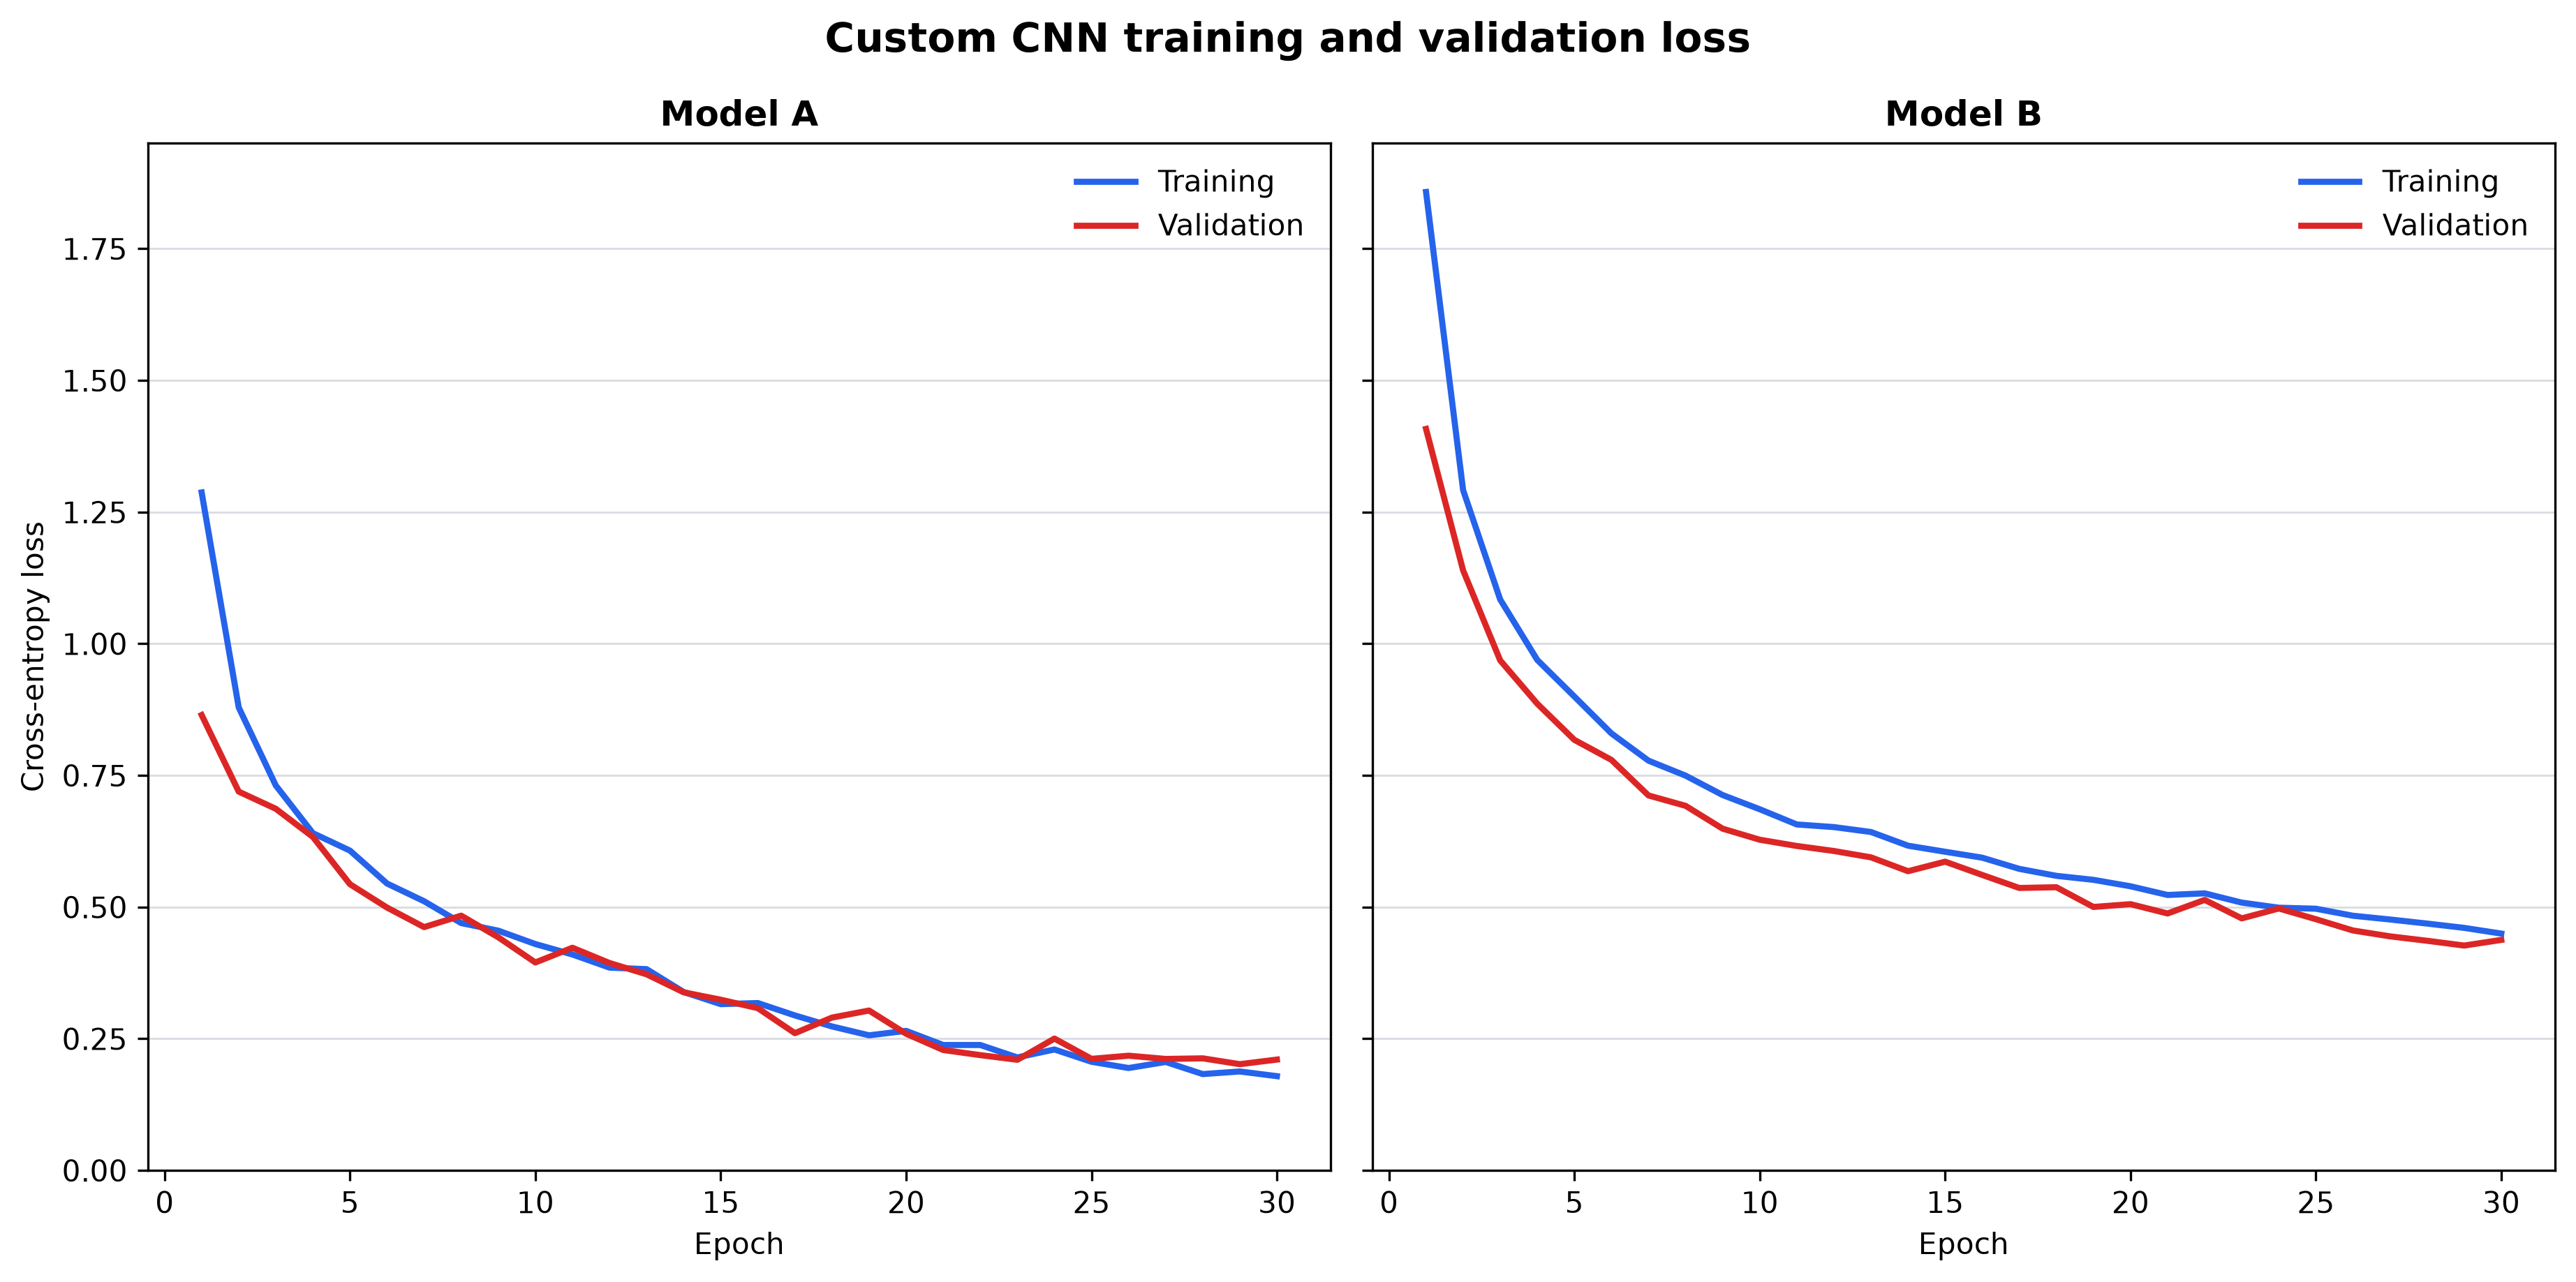
\includegraphics[width=\linewidth]{figures/custom_loss_curves.png}
  \caption{Training and validation cross-entropy loss for Model~A and
  Model~B.  The panels share a common vertical scale.}
  \label{fig:custom-loss}
\end{figure}

\begin{table}[htbp]
  \centering
  \small
  \resizebox{\linewidth}{!}{\begin{tabular}{lrrrrrr}
\hline
Model & Parameters & Size (KB) & Epoch (s) & Accuracy (\%) & Precision (\%) & Recall (\%) \\
\hline
Model A & 692{,}106 & 2{,}708.06 & 11.80 & 92.89 & 93.20 & 92.52 \\
Model B & 36{,}968 & 150.98 & 11.61 & 83.75 & 83.30 & 83.42 \\
\hline
\end{tabular}
}
  \caption{Custom-model comparison generated from the committed test metrics
  and profiler outputs.  Precision and recall are macro averages over the ten
  EuroSAT classes; epoch time was measured on the same Tesla T4.}
  \label{tab:custom-comparison}
\end{table}

Table~\ref{tab:custom-comparison} shows the central resource--accuracy
trade-off.  Replacing standard convolutions with depthwise and pointwise steps,
and replacing the flattened classifier input with global average pooling,
makes Model~B dramatically smaller while giving up some test accuracy, macro
precision, and macro recall.  The reduced capacity is most visible for
visually overlapping land-cover categories: Figure~\ref{fig:model-b-confusion}
shows more confusion among Herbaceous Vegetation, Permanent Crop, Highway,
and River than Figure~\ref{fig:model-a-confusion}.  In contrast, both models
remain strong on classes with more distinctive appearance, including Forest,
Residential, and Sea/Lake.

\subsubsection{Convergence control}

The 30-epoch comparison controls the early training budget, but its loss curve
shows that Model~B had not converged.  To separate convergence speed from
architecture capability, both models were therefore repeated for 100 epochs
with otherwise identical configurations.  The first 30 loss and accuracy
records reproduce the original runs exactly (apart from wall-clock noise), so
this is a controlled extension rather than a new hyperparameter search.

\begin{figure}[htbp]
  \centering
  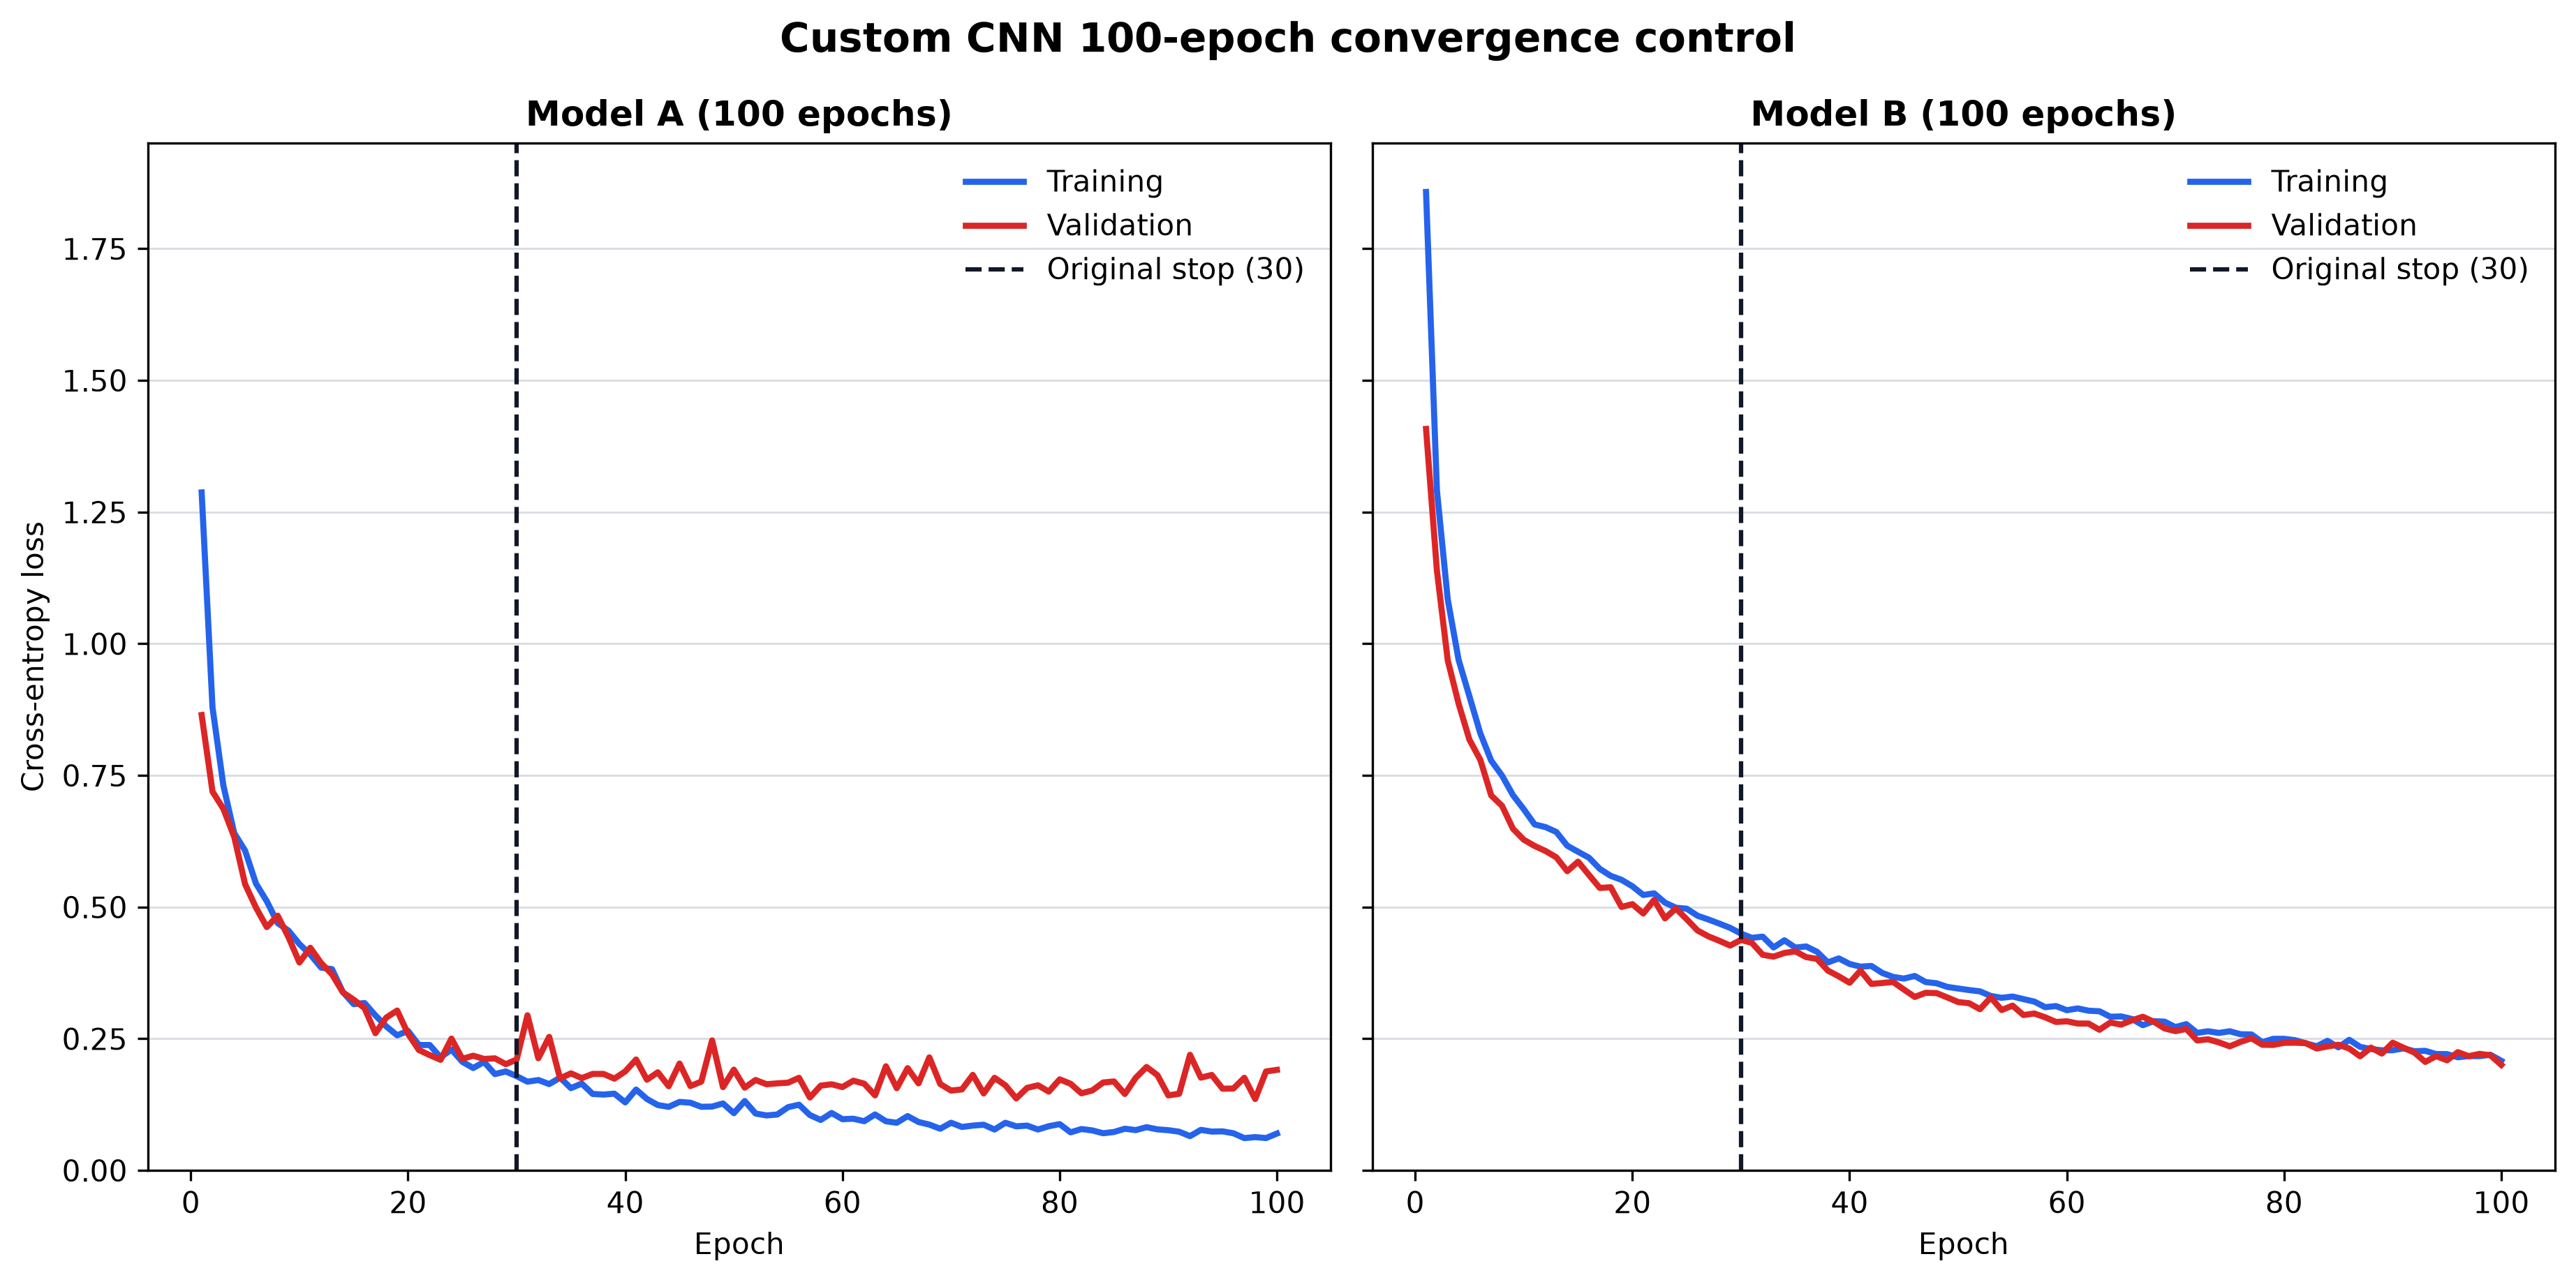
\includegraphics[width=\linewidth]{figures/custom_convergence.png}
  \caption{One-hundred-epoch training and validation loss for both custom
  models.  The dashed line marks the original 30-epoch stopping point.}
  \label{fig:custom-convergence}
\end{figure}

\begin{table}[htbp]
  \centering
  \scriptsize
  \resizebox{\linewidth}{!}{\begin{tabular}{lrrrrrrrrr}
\hline
Model & Epochs & Selected & Best val. loss & Best val. acc. (\%) & Test acc. (\%) & Parameters & Size (KB) & MACs & Epoch (s) \\
\hline
Model A & 30 & 29 & 0.2018 & 93.43 & 92.89 & 692{,}106 & 2{,}708.06 & 30{,}038{,}016 & 11.80 \\
Model A & 100 & 98 & 0.1355 & 96.00 & 96.00 & 692{,}106 & 2{,}708.06 & 30{,}038{,}016 & 12.54 \\
Model B & 30 & 29 & 0.4270 & 84.42 & 83.75 & 36{,}968 & 150.98 & 3{,}725{,}196 & 11.61 \\
Model B & 100 & 100 & 0.2004 & 93.26 & 93.14 & 36{,}968 & 150.98 & 3{,}725{,}196 & 12.29 \\
\hline
\end{tabular}
}
  \caption{Controlled custom-model convergence comparison.  ``Selected'' is
  the lowest-validation-loss checkpoint; all timings were measured on the
  same Tesla T4.}
  \label{tab:custom-convergence}
\end{table}

Table~\ref{tab:custom-convergence} shows that longer training benefits
Model~B much more strongly, substantially narrowing the accuracy gap without
changing its parameter, storage, or MAC advantage.  The two tables answer
different questions: Table~\ref{tab:custom-comparison} measures performance
under the same early epoch budget, whereas Table~\ref{tab:custom-convergence}
measures the architectures after a longer equal budget.  The former must not
be presented as Model~B's converged capability.

Model~A shows mild late-stage overfitting: its training loss continues to
fall while validation loss plateaus and fluctuates.  Selecting the
lowest-validation-loss checkpoint at epoch 98 mitigates that deterioration,
and the matching validation and test accuracies support good generalisation
of the selected checkpoint.  Model~B selects the final epoch, so even the
100-epoch result should be described as the achieved result, not a proven
upper limit on the architecture.

\begin{figure}[htbp]
  \centering
  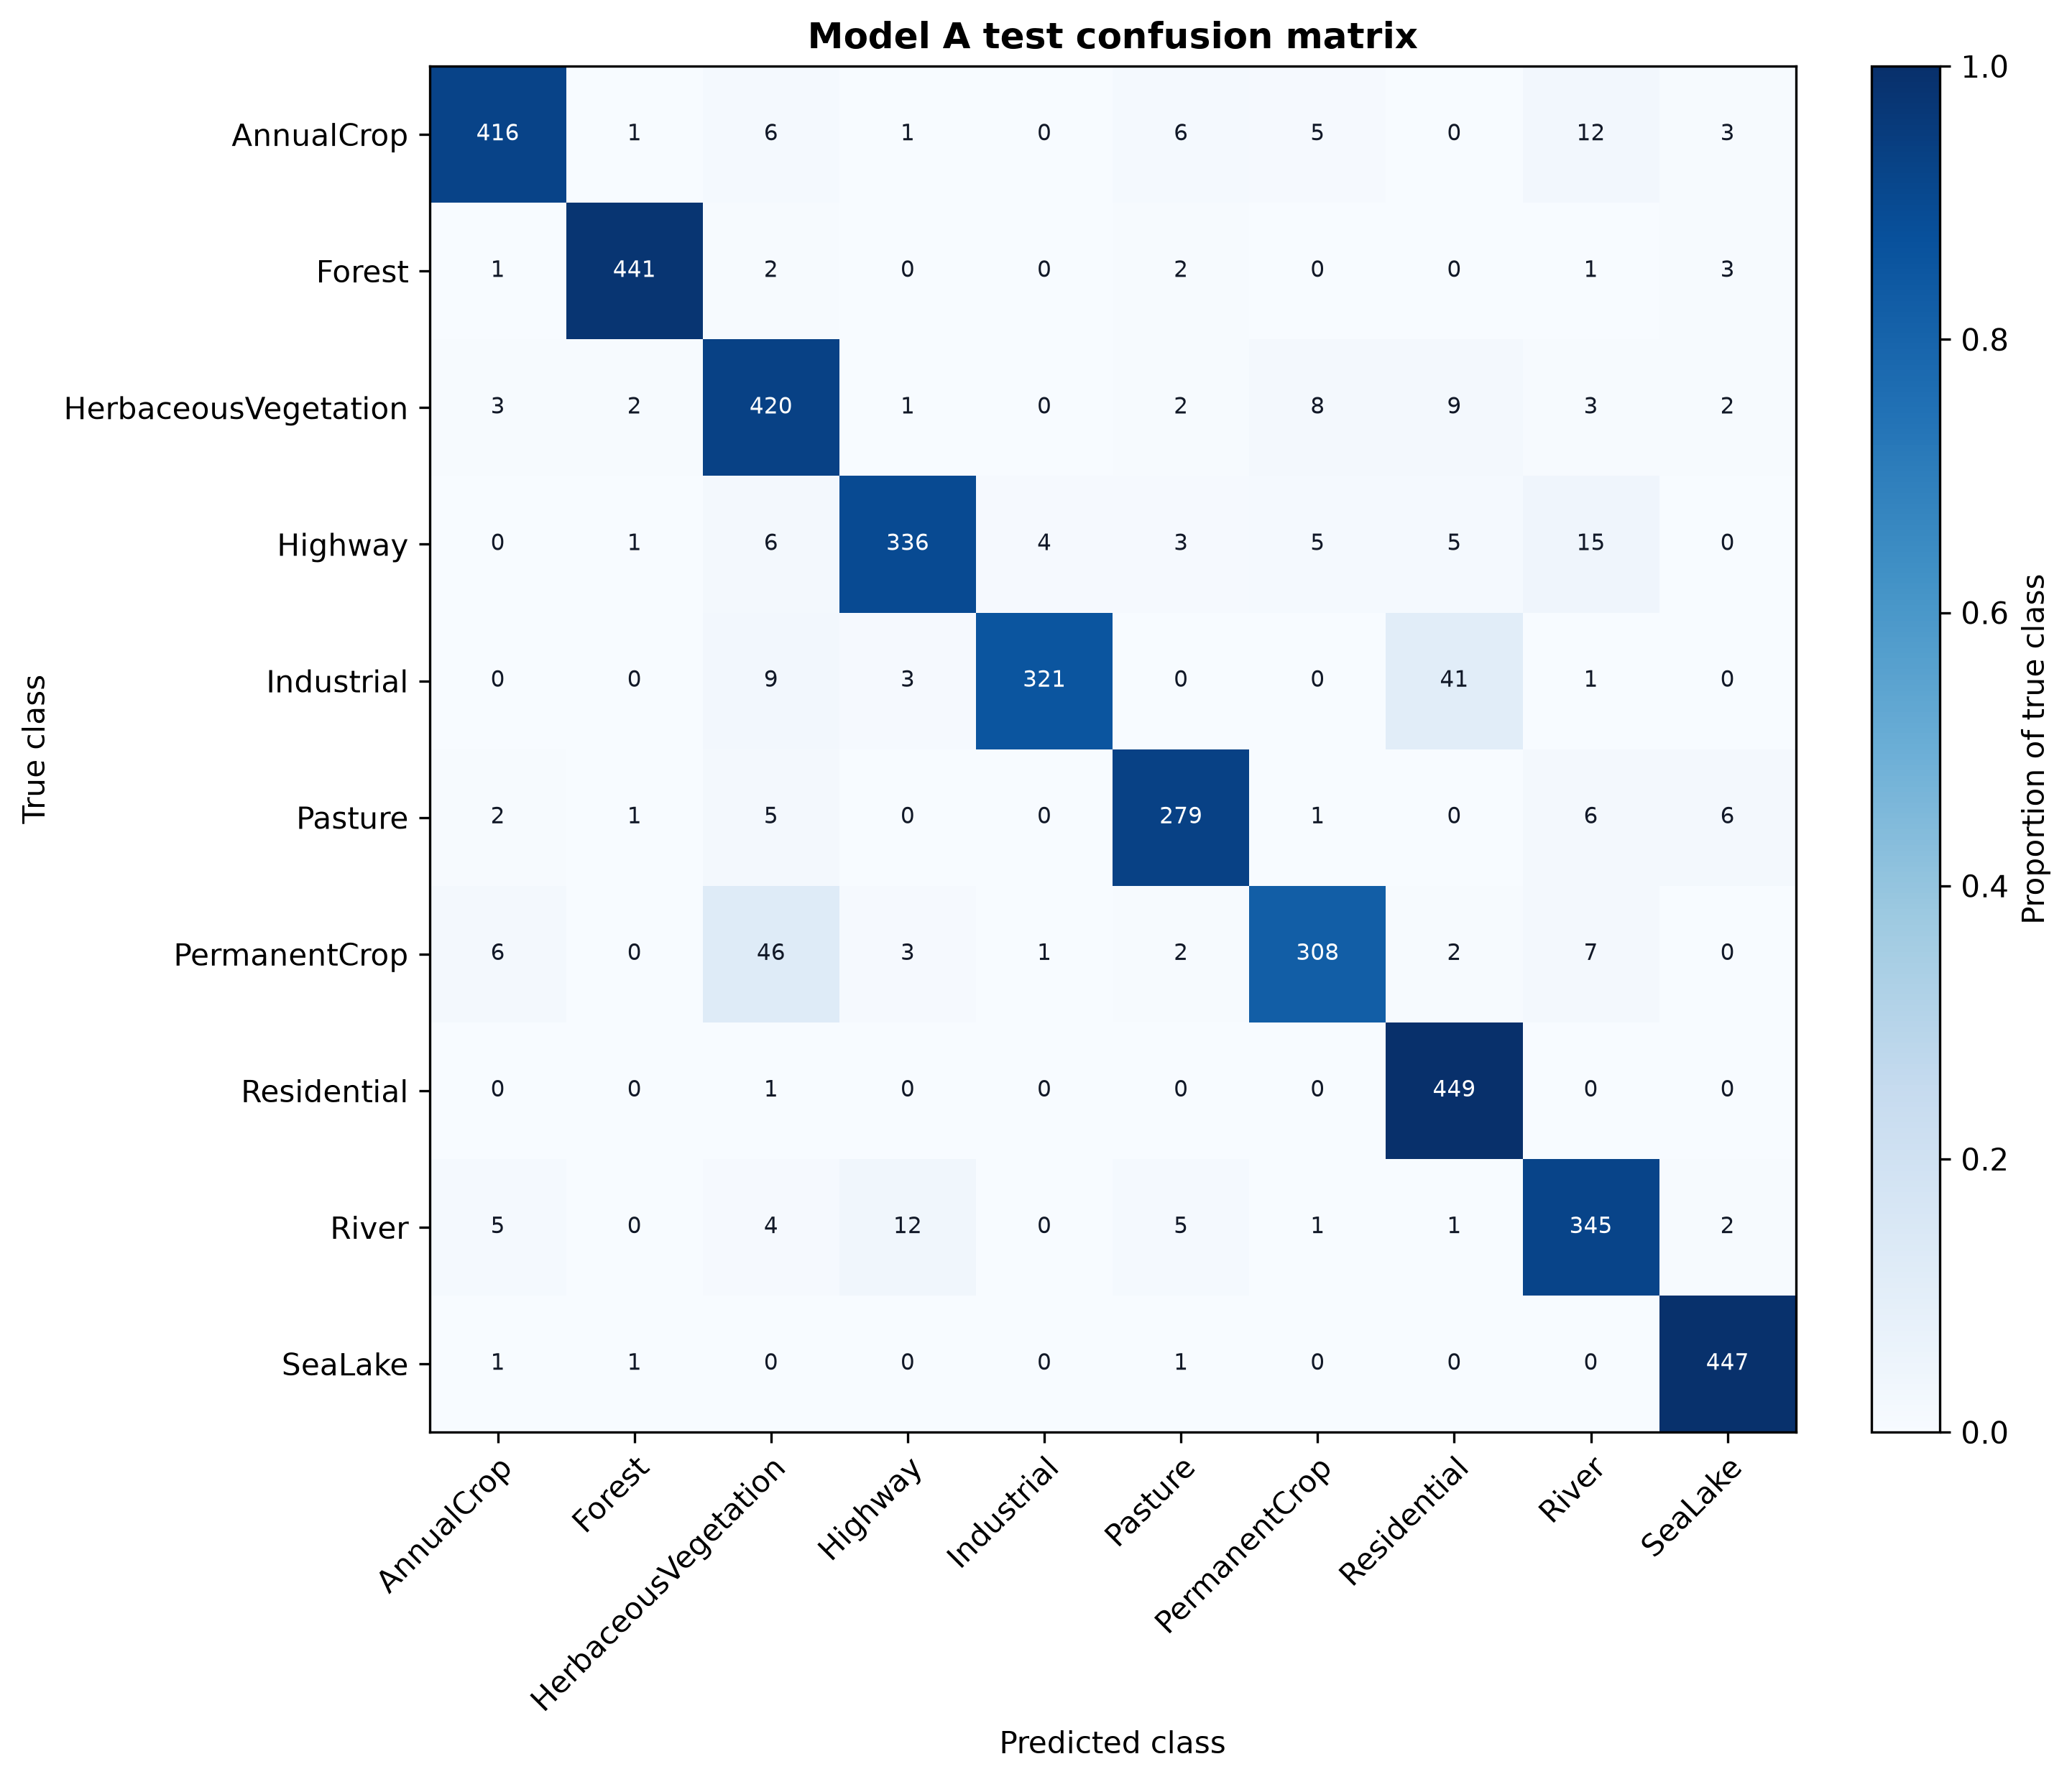
\includegraphics[width=0.82\linewidth]{figures/model_a_confusion_matrix.png}
  \caption{Model~A test confusion matrix.  Colour is normalised within each
  true-class row and annotations give raw sample counts.}
  \label{fig:model-a-confusion}
\end{figure}

\begin{figure}[htbp]
  \centering
  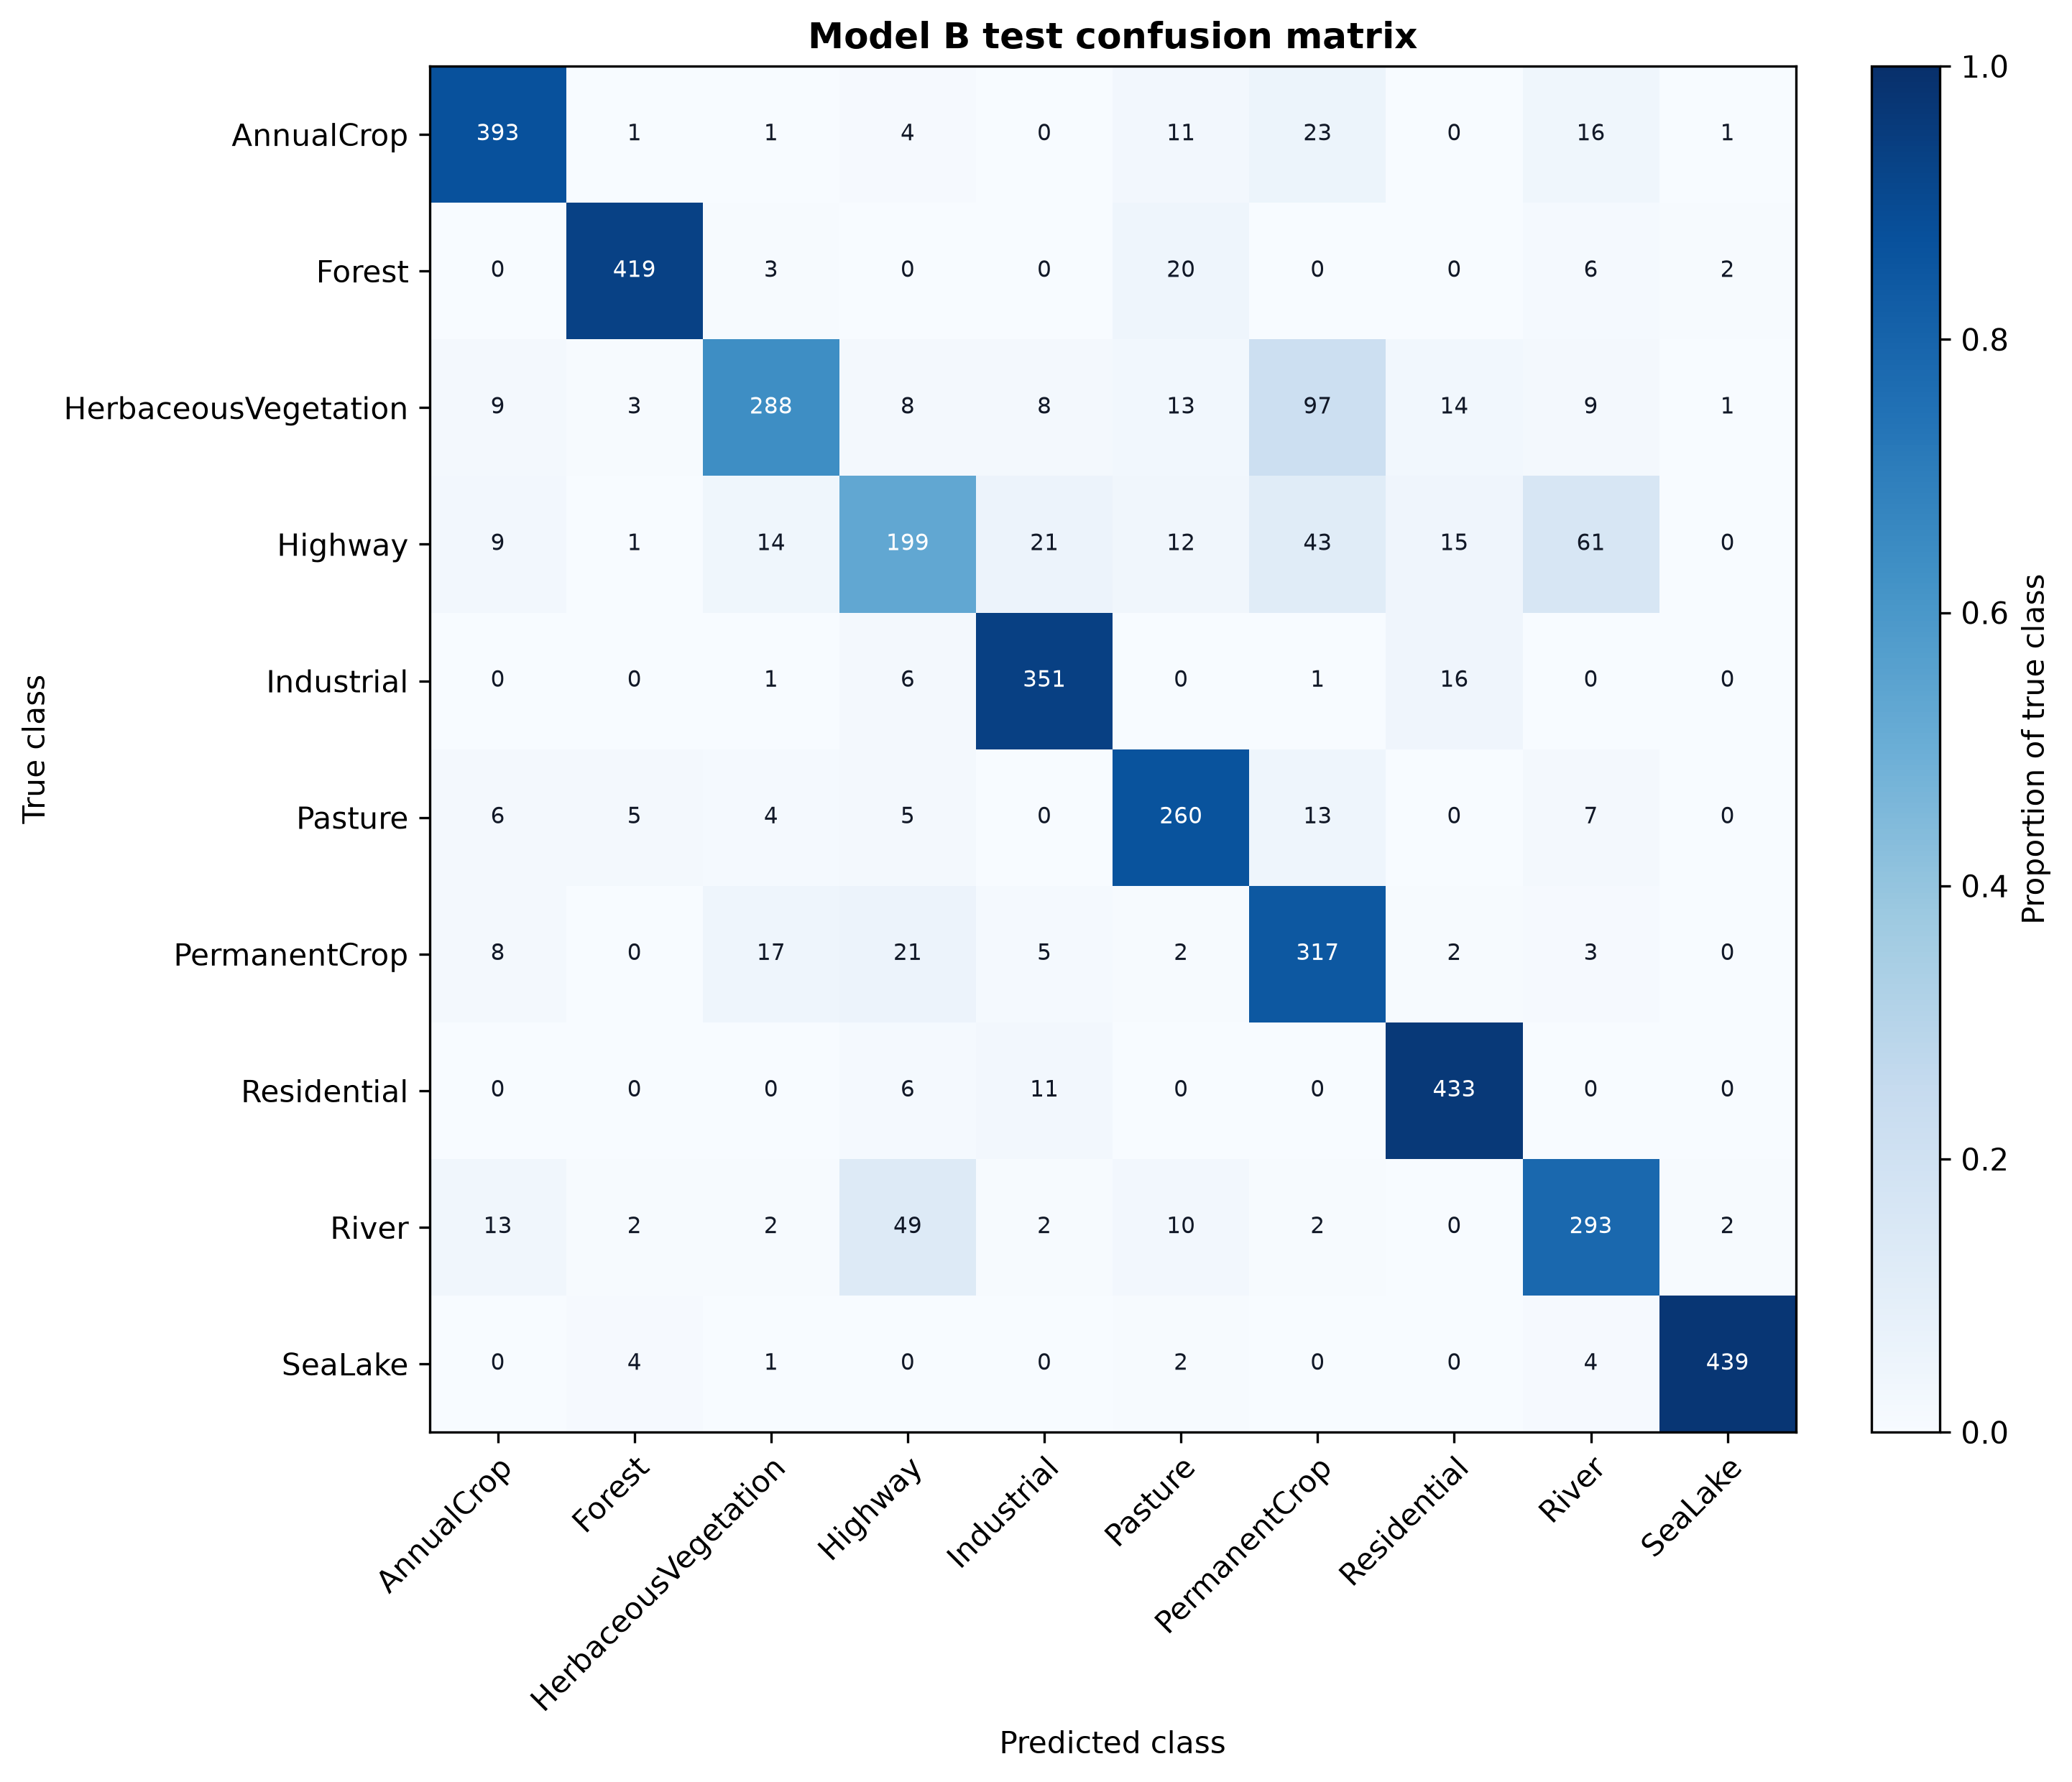
\includegraphics[width=0.82\linewidth]{figures/model_b_confusion_matrix.png}
  \caption{Model~B test confusion matrix, using the same convention as
  Figure~\ref{fig:model-a-confusion}.}
  \label{fig:model-b-confusion}
\end{figure}

The storage saving is substantial, but the epoch-time reduction is small.
This is not a contradiction: the profiler counts arithmetic, whereas wall-clock
training also includes data loading, augmentation, framework overhead, memory
traffic, and the efficiency of the accelerator's particular convolution
kernels.  Depthwise convolution reduces theoretical work without guaranteeing
the same proportional speed-up on a highly parallel GPU.  Its benefit is
clearer under the assignment's edge constraint, where the much smaller
parameter footprint and lower MAC count directly reduce storage and inference
work.  Model~A is preferable when predictive performance is the priority;
Model~B is the defensible choice when the parameter ceiling and deployability
are hard constraints.
